\documentclass[]{article}
\usepackage[T1]{fontenc}
\usepackage[pdftex,bookmarks=true,bookmarksnumbered=true,pdfauthor={Urs Reupke},pdftitle={Anathema Installation Guide}]{hyperref}
\usepackage[pdftex]{graphics}
\usepackage{graphicx}
\usepackage{textcomp}

\title{Anathema Installation Guide\\ Target Program Version: 1.0}
\author{Anathema created by Sandra Sieroux and Urs Reupke}
\date{}

\begin{document}
\sffamily
\maketitle
\tableofcontents
\bigskip
Two years in the making, version 1.0 of Anathema is finally upon us. Among other features, it brings a redesign of the foundations of the program. I took this as a chance of rewriting the year-old download system, as well as revising the present guide. 

I hope for this guide to answer all question that arise during download, installation and configuration of Anathema. All you require are a standard issue PC, internet access and basic computer skills.

I have tried to keep the guide independent of operating system specialties - and I failed spectacularly. If anything does not work as written or needs further clarification for a specific system, please let me know. This is especially true of Mac OS X, which I have never even touched. A plethora of contact options is provided at the Anathema website\footnote{http://anathema.sf.net}. You can also mail me directly\footnote{urskr@users.sf.net}.
\begin{flushright}
Enjoy Anathema\\
	-Urs
\end{flushright}
\section{System requirements}
While Anathema does not demand anything special in terms of hardware, there is some software that is required to run the program or at least necessary to make the most out of it.

First of all, Java. Anathema is written in the Java programming language and thus needs a working installation of the Java Runtime Environment to run. The minimum Java version required is version 5.0.

If you are already using Java, you can find out what version you are running by opening a console window and typing \texttt{java --version} followed by the \textsc{Enter} key. The resulting output should look something like this:
\medskip
\newline
\small
\texttt{java version "1.5.0\_06"
\newline
Java(TM) 2 Runtime Environment, Standard Edition (build 1.5.0\_06-b05)
\newline
Java HotSpot(TM) Client VM (build 1.5.0\_06-b05, mixed mode)}
\medskip
\newline
\normalsize
The version in this case, repeated in each line, is ``1.5.0\_06''. The relevant digit in our case is the second one: If it is 5 or greater, you're fine.

If it reads lower than 5 or if you do not yet have a copy of the Java Runtime Environment installed, point your web browser to the Java website\footnote{http://java.com/en/download/manual.jsp}, where you can always download the latest version for free.
\medskip
\newline
In addition to Java, you might want a copy of Adobe Reader to view the documents produced. You can get it free of charge from Adobe\footnote{http://www.adobe.com/products/acrobat/readstep2.html}. Of course, any other program capable of displaying PDF files will suffice.

Finally, for greater enjoyment of the music library features, you will need an audio player capable of handling M3U-Playlists ( such as Winamp or XMMS).
\medskip
\newline
Now, with all of that behind us, let's get to the program itself.

\section{Which file to download?}
To download the latest version of Anathema, direct your browser to the Anathema project page\footnote{http://sf.net/projects/anathema} and look for the list of ``Latest File Releases''. Said list contains an entry for package \textsc{anathema}. Click that word, and a screen with a list of all versions released will open.

Note that releases come in two types, \emph{regular releases}, indicated by some Exalted-related name, and \emph{patches}, clearly designated by the word ``patch'' somewhere in the package name.
Regular releases are feature hefty, bringing new functionality and changes. Patches, on the other hand, fix what is broken in a prior release. 
Going from top to bottom, select the first version not labelled as a patch.

Mission accomplished? Great.

Know now that within each package are at least two flavours of Anathema: A \emph{raw} .zip archhive suitable for any operating system and a \emph{Mac OS X} .dmg file. These archive contain everything you need to run Anathema, that is the program itself and a flock of supportive files. 

Occasionally, there might be a third kind of archive, designated \emph{upgrade}. Don't worry about them now, we'll cover them in detail below.

To continue, simply choose the most appropriate package for your operating system, and your download will start. While it is running, you could read on to familiarize yourself with the steps ahead or maybe have a look at our web site to learn about current proceedings.
\medskip

Once the download is finished, you are ready to proceed with the installation.

\subsection{Upgrades and Patches}
If this is your first experience with Anathema, please continue your installation and come back here later to upgrade.

Still there? Alright. So either we screwed up ($\rightarrow$ Patch) or there is cool new stuff to behold ($\rightarrow$ Upgrade). No matter what, your Anathema is outdated, and you want to change it. Here's how.

If there is a more recent version than the one on your system, but we didn't provide an upgrade archive, you will need to go through the installation procedure again. You can safely install the new files over the old installation, just make sure everything is properly overwritten.

If there is an upgrade, download it and extract the files into the old installation directory, overwriting existing files. \emph{Et voil\`a}, you are up to date again.

Upgrade archives are functionally identical to the \emph{raw} version, but are intended for those who already have a running copy of Anathema installed. Lacking the supporting files, they are meant as a way to update the previous version (which also might have been attained by means of upgrade) to the current one. They do not necessarily function with \emph{any} prior version. Not every package contains an upgrade.

Finally, if the new release is a patch, do as you would with an upgrade.As with upgrades, patch archives are not sufficient to run Anathema if it is not already installed and are clearly designated for use with a specific release.

No matter which of the three options it is, your saved files as well as previously made setting stay intact.

\section{Installation}
This step is really simple. Just unzip all the files within to an empty directory, using your favorite archive manager. Make sure that all relative path names are kept, lest Anathema misses some files.

Unless you are using Mac OS X, there is no automated installation mechanism. You will have to make your way to the directory manually, there to launch Anathema. 
\medskip

Let's continue the exploration by starting the program.

\section{Launching Anathema }
There are several ways of starting the program, depending on your operating system.

On most systems you can launch Anathema by opening a console window, changing to the Anathema directory and typing \texttt{java --jar anathema.jar}, followed by a stroke of \textsc{Enter}.
Windows users may opt to use the executable file anathema.exe that comes with the archive or type \texttt{javaw --jar anathema.jar} instead, but this will swallow any error reports that might come up during launch. Also, a freshly installed Java is configured to launch .jar files when they are double clicked in Windows.

A shell script, anathema.sh, is provided for Linux systems. Linux users should make sure that either read-- and write--access are granted on the Anathema directory or that a proper directory is specified at startup. See ``Command Line Options'' below for details.
  
\subsection{Command Line Options}
To submit any optional command line parameter to the launcher, you can put \linebreak
\texttt{-D\emph{[Name\_of\_Option]}} between \texttt{java} and the final argument \texttt{-jar anathema.jar}. Currently, this is only used to supply a custom repository directory.

\begin{description}
\item[repository] - Specifies the directory to use for storage and retrieval. If the directory given does not exist, it will be created if necessary read/write--permissions are granted. If the parameter is omitted, a subdirectory ``Repository'' in the main Anathema folder is assumed to be the repository directory.

	Example:\newline
	\texttt{java -Drepository="C:$\backslash$AnathemaRepository" -jar anathema.jar} will instruct Anathema to store and retrieve data from the directory 
	\linebreak``C:$\backslash$AnathemaRepository''.
	
For future launches, a more permanent way of setting the repository directory is provided. We'll address that in a minute.
\end{description}

\begin{figure}[htb]
	\centering
		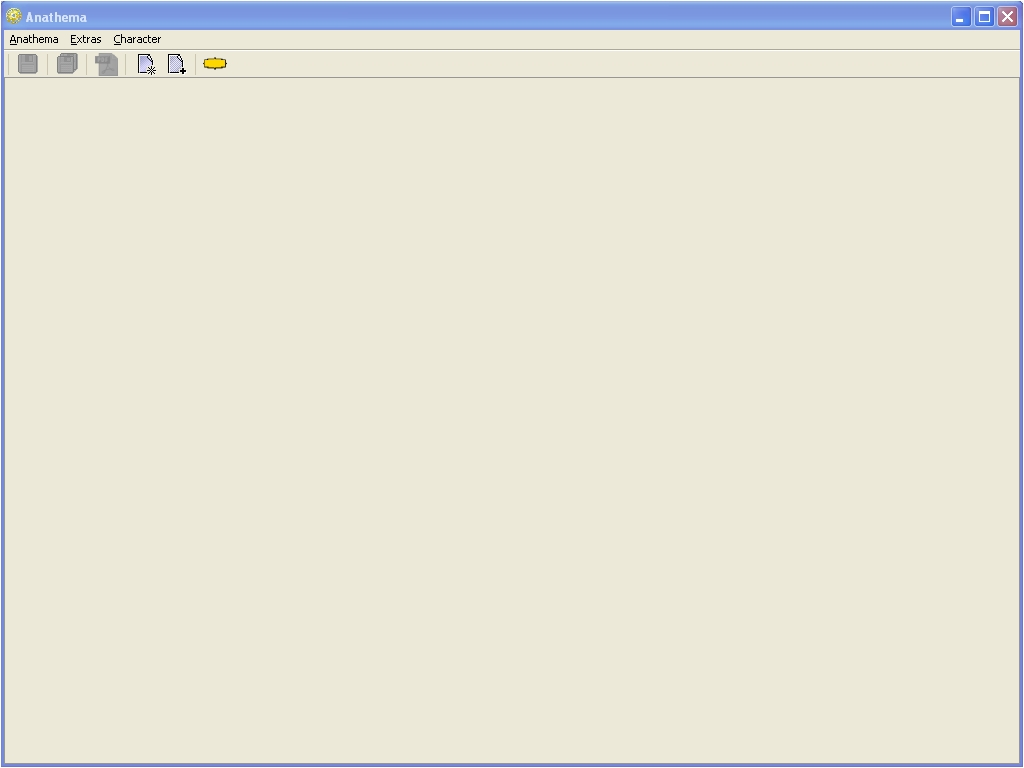
\includegraphics[width=1.00\textwidth]{Images/MainWindow.jpg}
	\caption{The Main Window, Windows Look \& Feel}
	\label{fig:MainWindow}
\end{figure}

\begin{figure}[htb]
	\centering
		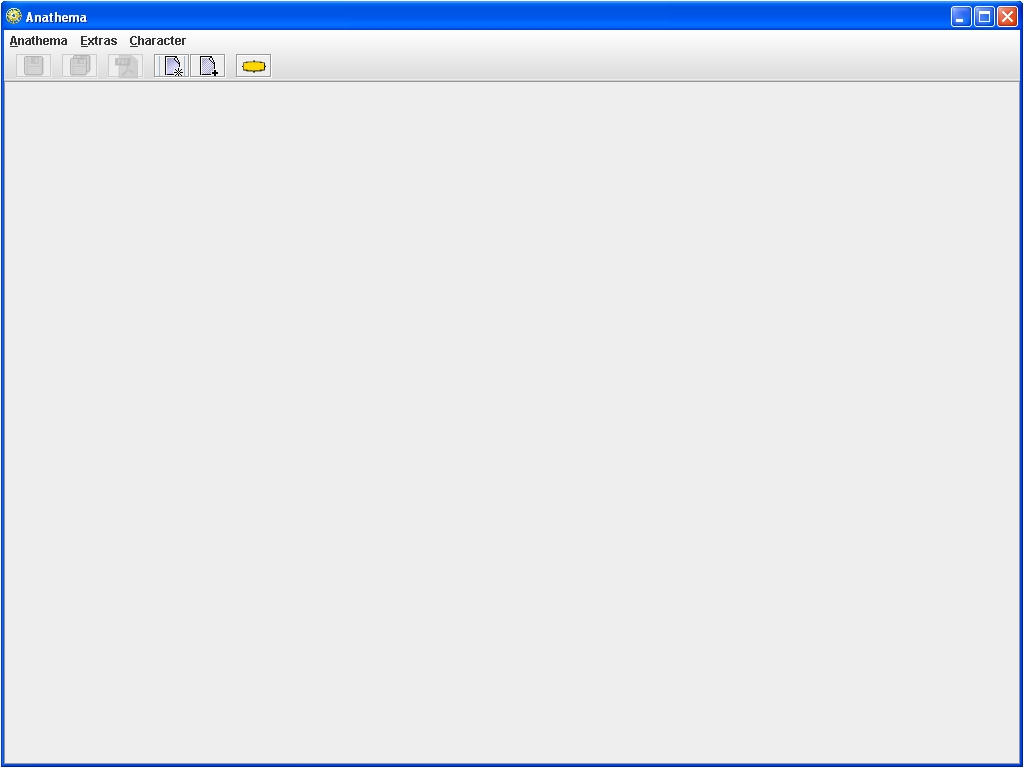
\includegraphics[width=1.00\textwidth]{Images/MainWindowMetal.jpg}
	\caption{The Main Window, Metal Look \& Feel}
	\label{fig:MainWindowMetal}
\end{figure}

\subsection{Done!}
Regardless of the option you chose, Anathema will now load. After a moment's waiting, the splash screen should appear, shortly after to be replaced by the main window. The window on screen should now look similiar to figure \ref{fig:MainWindow} (Windows) or \ref{fig:MainWindowMetal} (everything else).

\textbf{Congratulations!} Your installation of Anathema is now ready to use. Go ahead, fool around! Enter all your favourite characters! Create a new one while you're at it!
\medskip
\newline
Once you're a tad more familiar with the program, come back here and learn about the various settings in the following section.

\section{Setting your Preferences}\label{sec:Preferences}
Tucked away in the menu \emph{Extras} is an entry called \emph{Preferences}. Clicking there unveils a dialog with - who would have thought - various options for Anathema's basic system. The options are stored on a per-user basis, so every account on your system can have it's own settings. Let's have a closer look:
\begin{description}
	\item[Use Metal Look \& Feel] - Available on Windows systems only. Checking the box forces Anathema to use the ``Metal Ocean'' controls instead of the more Windows-like ones used by default. Confer figures \ref{fig:MainWindow} and \ref{fig:MainWindowMetal} for a basic impression.
	\item[Launch maximized] - The Anathema window is maximized at launch. Useful on resolutions of 1024x768, where part of the window might be hidden by operating system controls at the screen's top and bottom.
	\item[Display document after print] - Controls whether PDF documents are opened in your system's default PDF viewer once printing is done.
	\item[Languange] - Selects the language to run the program in. Currently, English and Spanish are available.
	\item[Show tooltips for (seconds)] - This setting, while global, is mainly intended to control the time until displayed Charm details vanish. 
	\item[Repository directory] - The aforementioned option to permanently set the infamous repository directory. Enter a directory or click the browse button for a graphical selection interface. If the directory does not exist, no changes are made to the setting.
\end{description}
	
When everything is set, click \emph{OK} to commit your changes. A dialog will kindly inform you that you need to restart Anathema to see the effects of any changes. You can do so now or at any later point in time. If you clicked \emph{Cancel} instead, the preferences dialog will vanished and all changes are undone.
\medskip
\newline
This concludes the tour of the Anathema setup.

I hope you enjoy the program and stay with us to experience plenty of new versions and features ahead.
\medskip
\newline
Thank you for using Anathema.

\begin{appendix}
\section*{Revisions}
\begin{description}
\item[10/22/06] - Revision for v1.0
\item[08/14/05] - Initial Release for v0.8
\end{description}
\end{appendix}
\end{document}